\documentclass{beamer}
% \usetheme{metropolis}
\usefonttheme{structuresmallcapsserif}
\usepackage{times}

\title{Linear Regression: Validation}
\author{Connor K. Brubaker}
\institute{
Department of Statistics \\
Texas A\&M University
}
\date{}

\begin{document}
\maketitle

\begin{frame}{Model Validation}
    Inferences and predictions made from a fitted model only make sense if the assumptions of that model are fulfilled.

    \vspace{1em}
    Model validation is the process of evaluating if the assumptions are met.
\end{frame}

\begin{frame}{Anscombe’s Data Sets}
    \begin{center}
        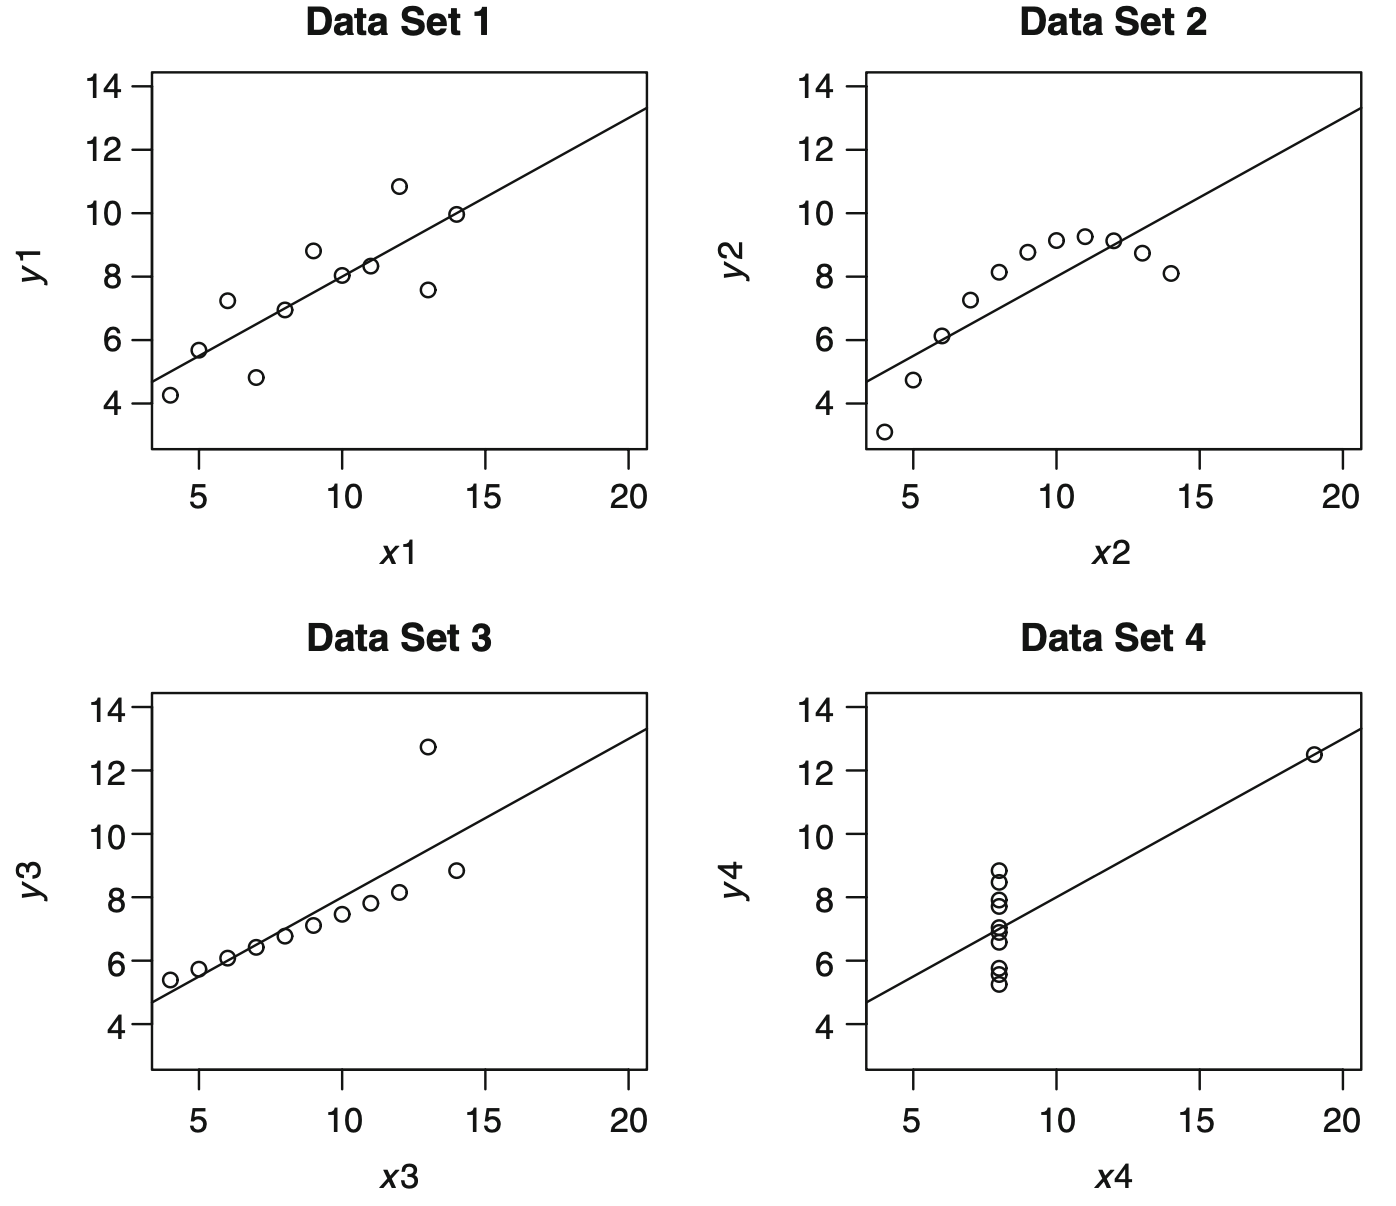
\includegraphics[width=.75\linewidth]{figures/Anscombe.png}
    \end{center}
\end{frame}

\begin{frame}{Anscombe’s Data Sets}
    Each of these four data sets results in the same fitted regression line,
    \begin{equation*}
        \hat{Y} = 3 + 0.5 X
    \end{equation*}
    but only one (Data Set 1) satisfies the assumptions of the model--only one of these results in a valid model! 

    \vspace*{1em}

    \textbf{Don't just look at numerical output of a model. Always check it visually!}
\end{frame}

\begin{frame}{Assumptions of the Linear Model}
    The simple linear model makes four assumptions:
    \begin{enumerate}
        \item $X$ and $Y$ are linearly related,
        \item the errors $\varepsilon_1, \ldots, \varepsilon_n$ are independent of each other,
        \item the errors $\varepsilon_1, \ldots, \varepsilon_n$ have a common variance $\sigma^2$ (homoscedasticity), and 
        \item the errors $\varepsilon_1, \ldots, \varepsilon_n$ are normally distributed with a mean of $0$ and variance $\sigma^2$.
    \end{enumerate}
    We will look at ways of visually evaluating these.
\end{frame}

\begin{frame}{Linearity and Constant Variance}
    Linearity and homoscedasticity is assessed by looking at scatter plots of the fitted residual 
    \begin{equation*}
        \hat{\varepsilon}_i = Y_i - \hat{Y}_i
    \end{equation*}
    against $X_i$ (called a residual plot). 

    \vspace{1em}

    A residual plot should have no discernable pattern.
\end{frame}

\begin{frame}{Residual Plots for Anscombe’s Data Sets}
    \begin{center}
        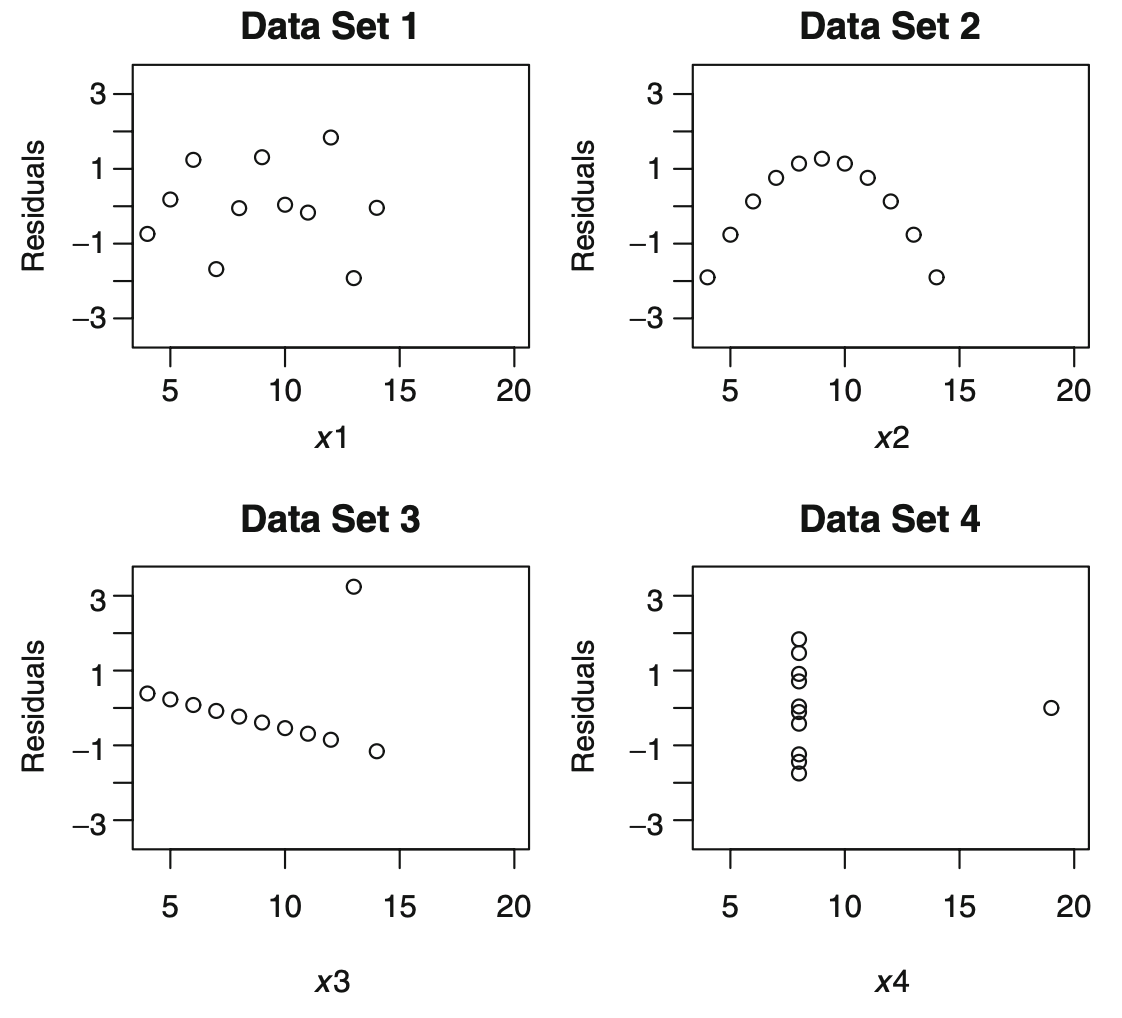
\includegraphics[width=.75\linewidth]{figures/anscombe-resid.png}
    \end{center}
\end{frame}

\begin{frame}{Residual Plot for Housing Data}
    \begin{center}
        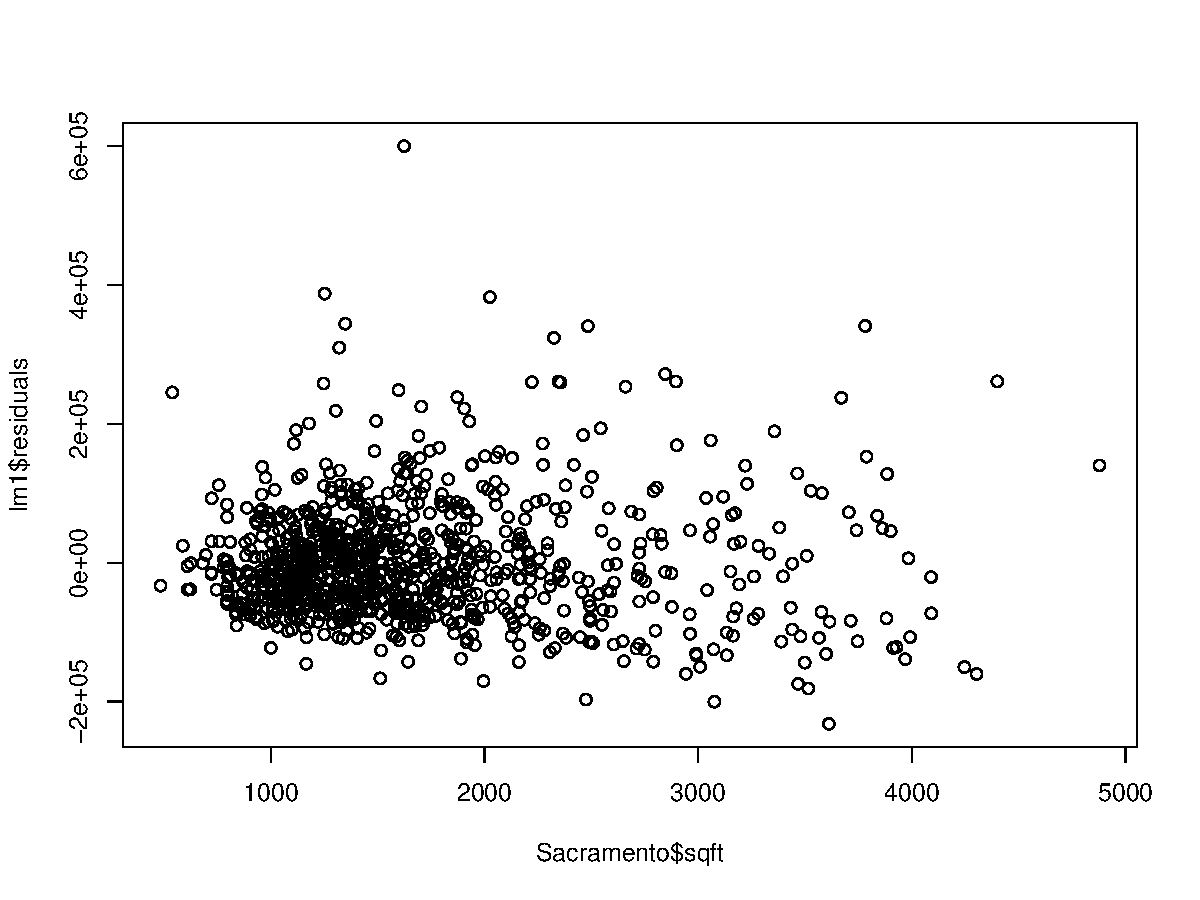
\includegraphics[width=.9\linewidth]{figures/housing-resid.pdf}
    \end{center}
\end{frame}

\begin{frame}{An Example of Heteroscedasticity}
    A residual plot like this indicates that the homoscedasticity assumption has been violated.
    \begin{center}
        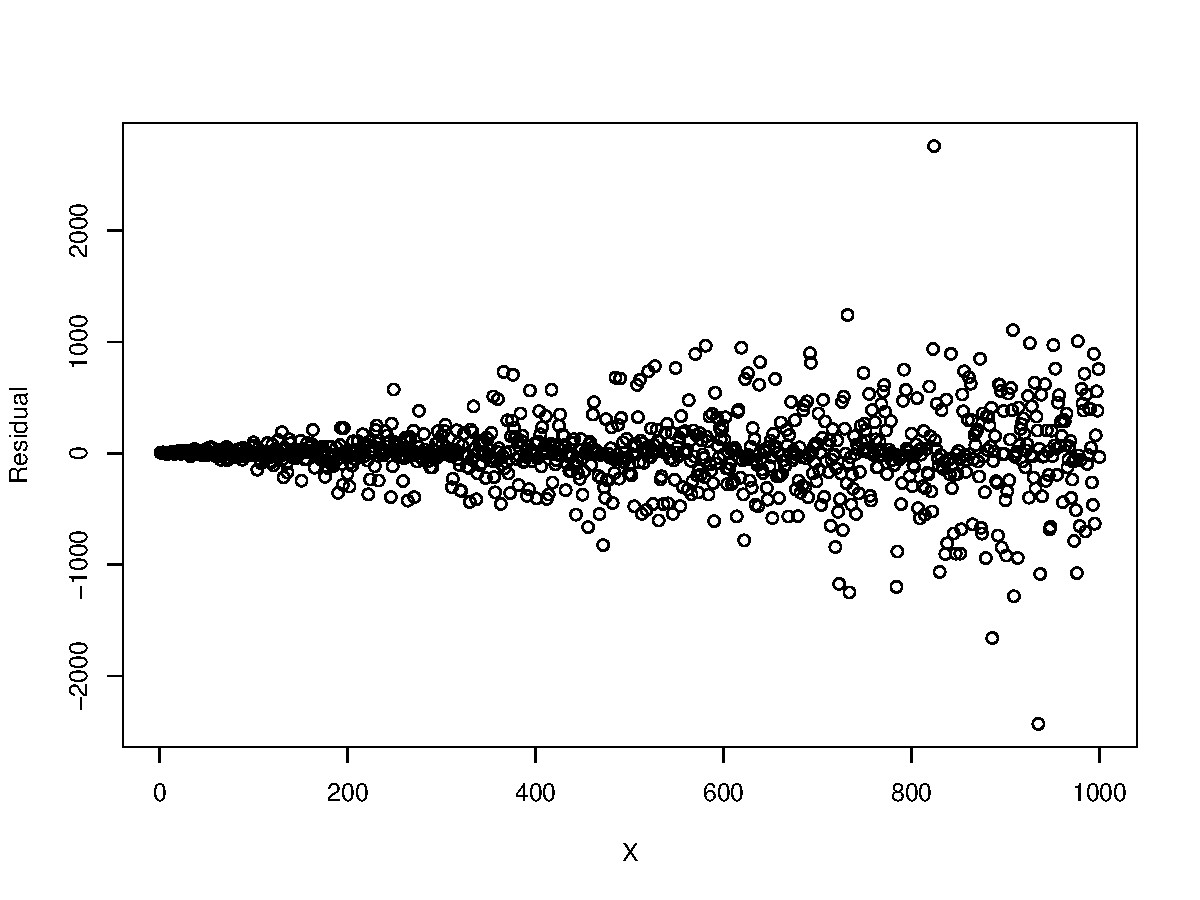
\includegraphics[width=.9\linewidth]{figures/heteroscedasticity.pdf}
    \end{center}
\end{frame}

\begin{frame}{Normality Assumption}
    The normality of errors assumption can be checked visually with a normal Q-Q plot like we've seen before. Here is the Q-Q plot of the residuals from the housing data.
    \begin{center}
        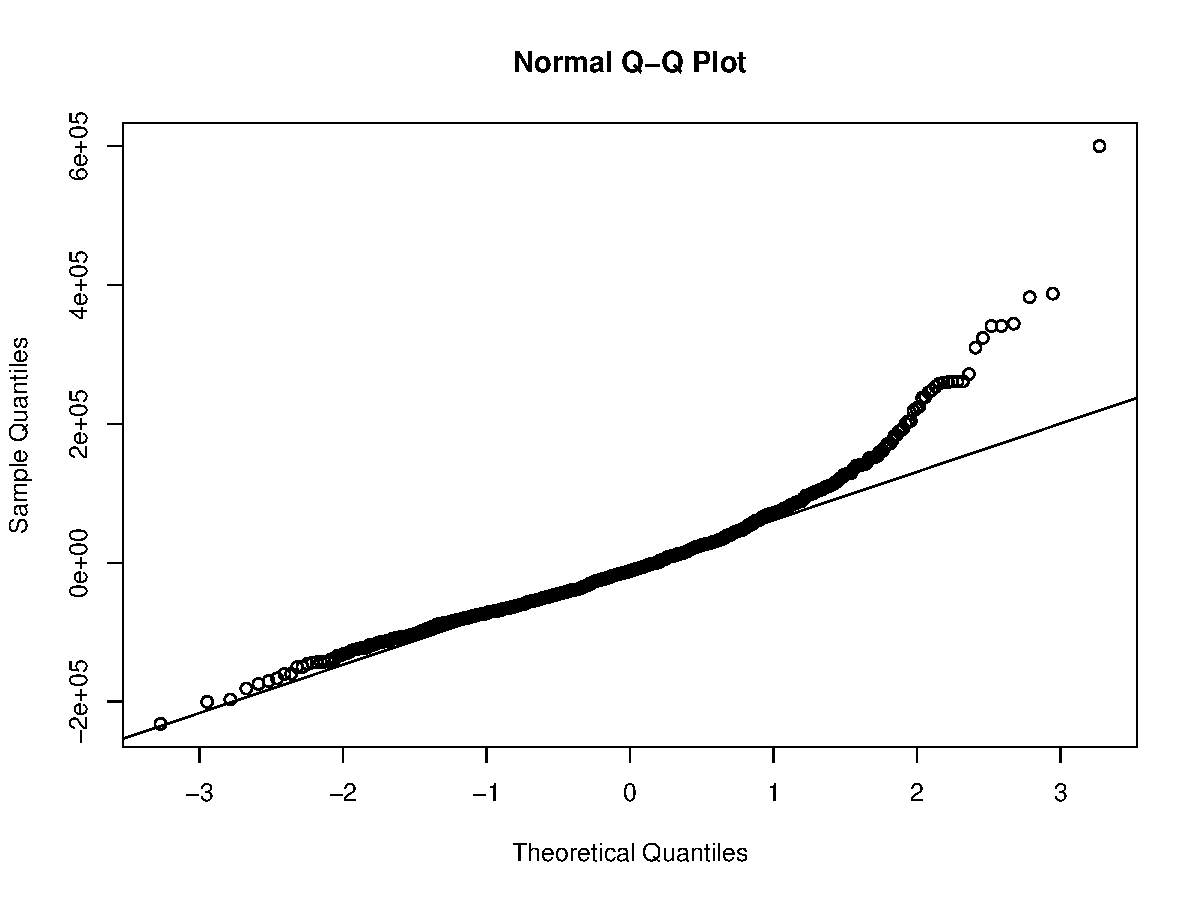
\includegraphics[width=.8\linewidth]{figures/housing-qq.pdf}
    \end{center}
\end{frame}

\begin{frame}{Leverage Points}
    \begin{itemize}
        \item Data points which have considerable influence on the fitted model are called \textbf{leverage points}. 
        \item They have $X$ values that lie away from the rest of the data points. 
        \item Leverage points can be either ``good'' or ``bad''.
        \item The leverage of a point can be examined by removing it from the data, refitting the model, and evaluating the effect. 
    \end{itemize}
\end{frame}

\begin{frame}{Good Leverage Points}
    A leverage point that follows the linear pattern of the data is a good leverage point. 
    \vspace*{-1em}
    \begin{center}
        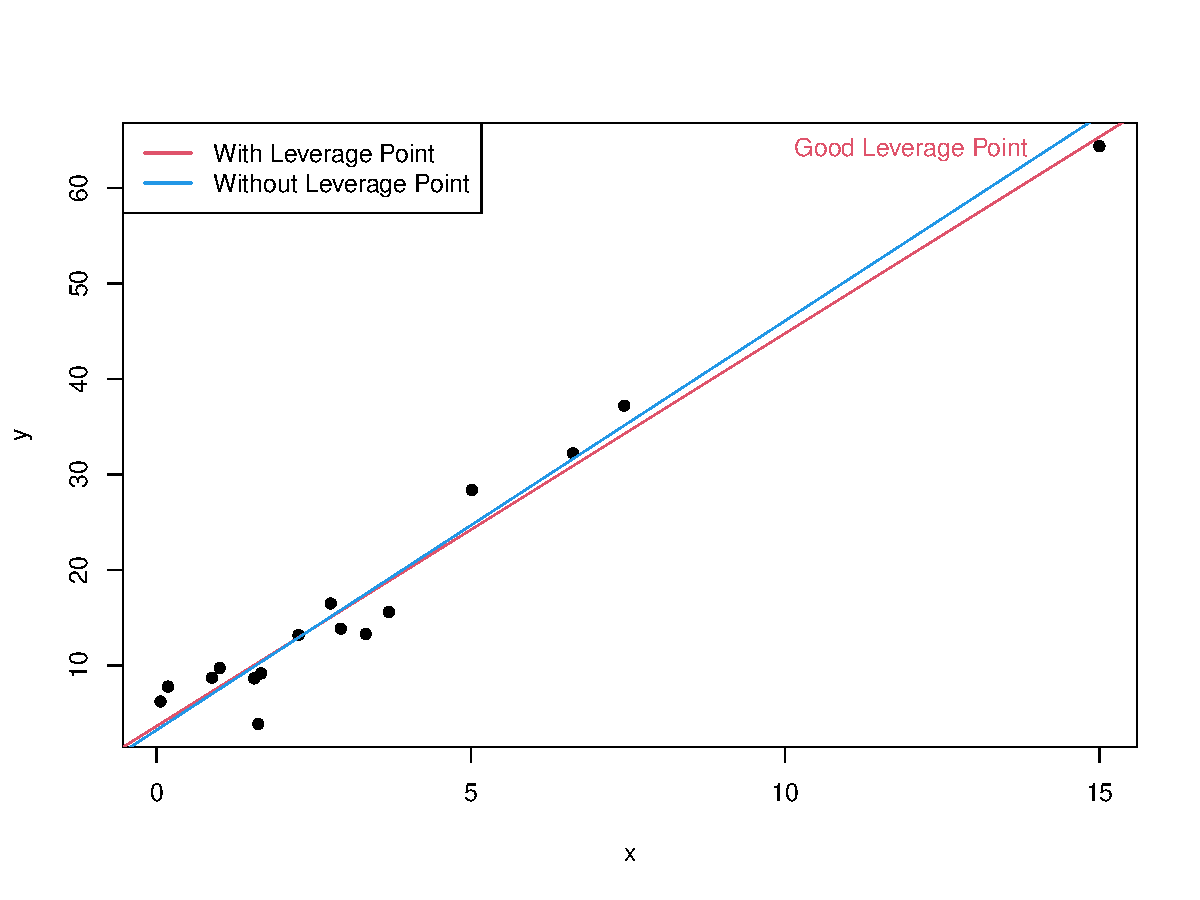
\includegraphics[width=.9\linewidth]{figures/good_leverage.pdf}
    \end{center}
\end{frame}

\begin{frame}{Good Leverage Points}
    A leverage point that is also an outlier is a bad leverage point.
    \vspace*{-1em}
    \begin{center}
        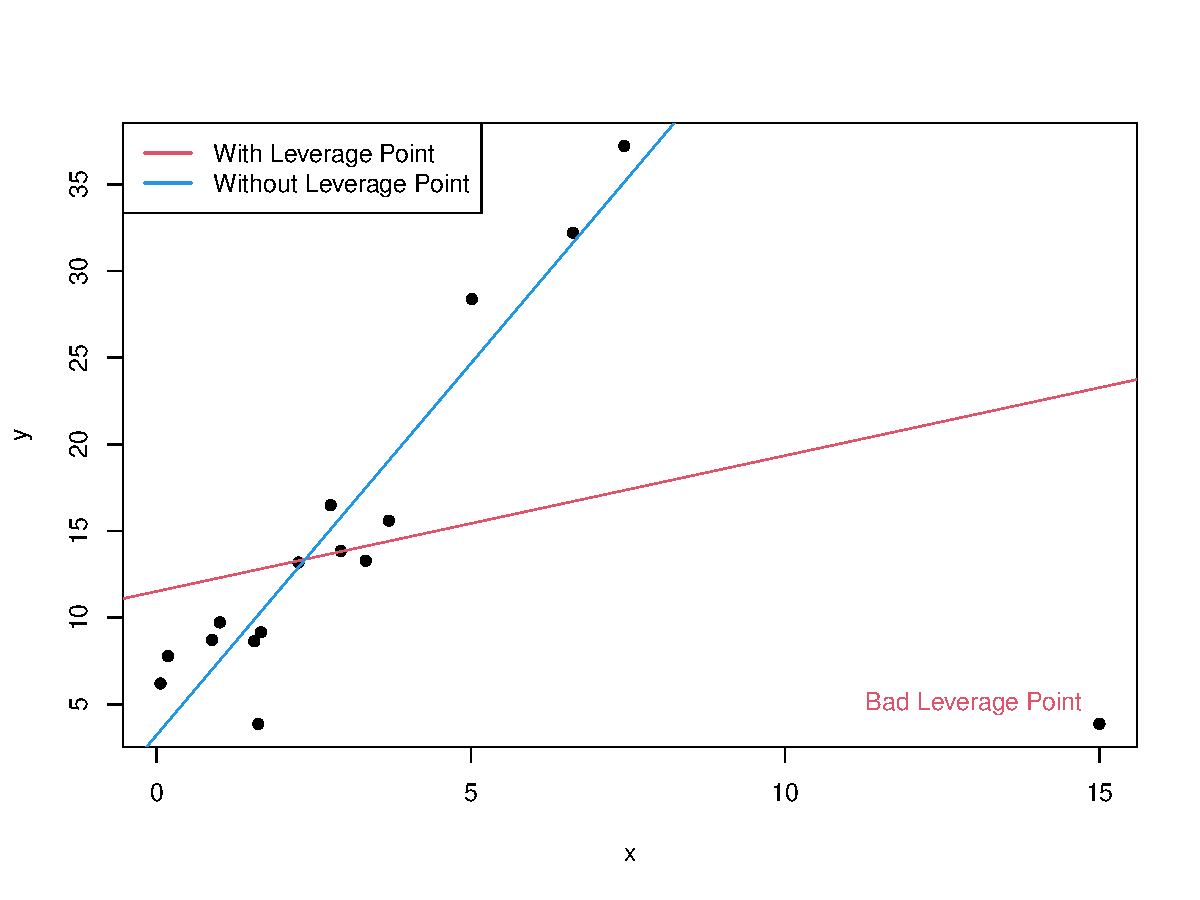
\includegraphics[width=.9\linewidth]{figures/bad_leverage.pdf}
    \end{center}
\end{frame}

\begin{frame}{Dealing With Bad Leverage Points}
    \begin{itemize}
        \item Bad leverage points need investigation. They may be candidates for removal from the data due to wrong data entry, bad experimental conditions, etc.
        \item If valid, the existence of bad leverage points may suggest a different model is needed (e.g., non-linear model)
        \item Even if a leverage point is ``good'', they do affect standard errors and the value of $R^2$, so they always warrant investigation to check they are valid.
    \end{itemize}
\end{frame}

\end{document}